%%%%%%%%%%%%%%%%%%%%%%%%%%%%%%%%%%%%%%%%%%%%%%%%%%%%%%%%%%%%%%%%%%%%%%
% Skupina01/main.tex -- VZOREC POGLAVJA
%
% Ta datoteka je primer, kako je poglavje zgrajeno. Kopirajte jo v svoj
% direktorij SkupinaXX, zamenjajte "g01:" z "gXX:" in besedilo v oglatih
% oklepajih [ ... ] nadomestite s svojim.
%
% Pravila:
%  - brez \usepackage (vse pakete naloži editor.tex),
%  - slike v SkupinaXX/img/, vse oznake in ključi virov z "gXX:",
%  - vire dodajte v skupno datoteko references.bib (z doi ali url).
%%%%%%%%%%%%%%%%%%%%%%%%%%%%%%%%%%%%%%%%%%%%%%%%%%%%%%%%%%%%%%%%%%%%%%

\graphicspath{{Skupina01/img/}}

\title{[Naslov seminarske naloge]}
% \titlerunning{[Krajši naslov]}  % če je naslov predolg za glavo strani
\author{[Ime Priimek], [Ime Priimek], [Ime Priimek] in [Ime Priimek]}
\maketitle

\abstract{[Povzetek v 5 do 10 vrsticah. Navedite raziskovalno vprašanje, uporabljeno metodo in orodja ter glavni rezultat s konkretno številko, npr.\ \enquote{Fizično reverzibilna izvedba polnega seštevalnika potrebuje 2,3-krat več celic in ima 1,5 urina cikla večjo zakasnitev kot ireverzibilna, disipira pa 40~\% manj energije.} Končajte z enim stavkom o pomenu rezultata.]}


\section{Uvod}
\label{g01:sec:uvod}

[Kratko predstavite področje (največ dve strani) in ga podprite z viri, npr.~\cite{lent1997} za kvantne celične avtomate ali~\cite{nielsen2010} za kvantno računanje. Opišite, kaj so drugi že naredili in kaj ostaja odprto.]

\begin{svgraybox}
\textbf{Raziskovalno vprašanje.} [Eno vprašanje, na katero bo poglavje odgovorilo z meritvijo, npr.\ \enquote{Pri koliko qubitih Groverjev algoritem na procesorju IBM ne da več uporabnega rezultata?}]

\textbf{Pričakovani rezultat.} [Vaša hipoteza pred začetkom dela.]
\end{svgraybox}

[Na koncu uvoda v nekaj stavkih opišite zgradbo poglavja.]


\section{Metode}
\label{g01:sec:metode}

\subsection{Orodja in nastavitve}
\label{g01:sec:orodja}

[Navedite orodja z različicami in vse nastavitve, ki vplivajo na rezultat, tako da lahko drugi poskus ponovijo. Tabela~\ref{g01:tab:parametri} je primer.]

\begin{table}[htbp]
\caption{Primer: parametri simulacije v QCADesigner-E. [Vpišite svoje vrednosti.]}
\label{g01:tab:parametri}
\centering
\begin{tabular}{lr}
\toprule
Parameter & Vrednost \\
\midrule
simulacijski model & [koherentni vektor] \\
temperatura & [\SI{1}{\kelvin}] \\
širina celice & [\SI{18}{\nano\metre}] \\
razdalja med središči celic & [\SI{20}{\nano\metre}] \\
urina shema & [USE] \\
\bottomrule
\end{tabular}
\end{table}

\subsection{Zasnova poskusov}
\label{g01:sec:poskusi}

[Opišite, katere poskuse ste izvedli in zakaj. Enačbe pišite v okolju \texttt{equation} in se nanje sklicujte, npr.\ polarizacija celice je določena z enačbo~\eqref{g01:eq:polarizacija}.]

\begin{equation}
P = \frac{(\rho_1 + \rho_3) - (\rho_2 + \rho_4)}{\rho_1 + \rho_2 + \rho_3 + \rho_4}
\label{g01:eq:polarizacija}
\end{equation}

[Za izris kvantnih vezij lahko uporabite paket \texttt{quantikz}. Slika~\ref{g01:fig:bell} je primer vezja, ki pripravi Bellovo stanje $\frac{1}{\sqrt{2}}(\ket{00} + \ket{11})$.]

\begin{figure}[htbp]
\centering
\begin{quantikz}
\lstick{$\ket{0}$} & \gate{H} & \ctrl{1} & \meter{} \\
\lstick{$\ket{0}$} & \qw      & \targ{}  & \meter{}
\end{quantikz}
\caption{Primer kvantnega vezja: priprava in merjenje Bellovega stanja.}
\label{g01:fig:bell}
\end{figure}

[Kratke odseke kode lahko vključite z okoljem \texttt{lstlisting}, celotno kodo pa hranite v repozitoriju.]

\begin{lstlisting}[language=Python, caption={Primer: izvedba vezja na kvantnem procesorju IBM.}, label={g01:lst:qiskit}]
from qiskit import QuantumCircuit
from qiskit.transpiler import generate_preset_pass_manager
from qiskit_ibm_runtime import QiskitRuntimeService, SamplerV2 as Sampler

qc = QuantumCircuit(2)
qc.h(0)
qc.cx(0, 1)
qc.measure_all()

backend = QiskitRuntimeService().least_busy(operational=True, simulator=False)
isa = generate_preset_pass_manager(backend=backend, optimization_level=1).run(qc)
job = Sampler(mode=backend).run([isa], shots=1000)
print(job.job_id(), job.result()[0].data.meas.get_counts())
\end{lstlisting}

\subsection{Metrike}
\label{g01:sec:metrike}

[Naštejte metrike, s katerimi odgovorite na raziskovalno vprašanje, in kako jih izračunate. Npr. število celic, površina, zakasnitev v urinih ciklih in disipacija energije za QCA. Verjetnost uspeha, globina vezja in število dvokubitnih vrat za QC.]


\section{Rezultati}
\label{g01:sec:rezultati}

[Rezultate predstavite s slikami, grafi in tabelami ter jih v besedilu razložite. Vsako sliko in tabelo omenite v besedilu, npr.\ slika~\ref{g01:fig:majoritetna} in tabela~\ref{g01:tab:primerjava}.]

\begin{figure}[htbp]
\centering
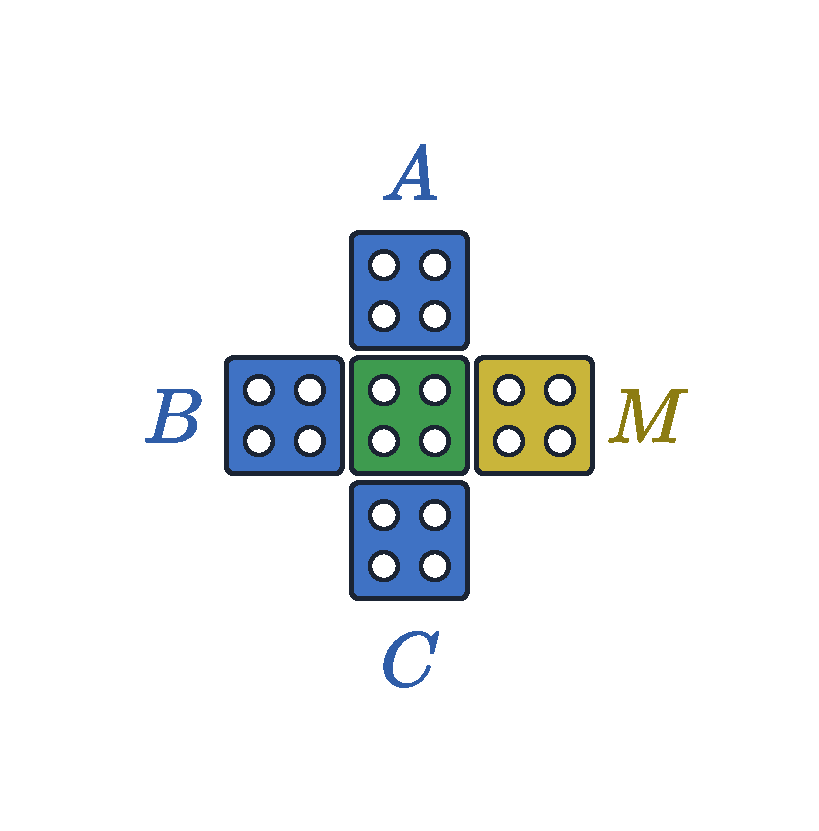
\includegraphics[width=0.4\textwidth]{majoritetna_vrata}
\caption{Primer slike: majoritetna vrata z vhodi $A$, $B$, $C$ in izhodom $M$. [Slike shranjujte v poddirektoriju \texttt{img} v formatu PDF ali PNG.]}
\label{g01:fig:majoritetna}
\end{figure}

\begin{table}[htbp]
\caption{Primer: primerjava lastne izvedbe z objavljenimi. [Vpišite svoje vrednosti in navedite vire.]}
\label{g01:tab:primerjava}
\centering
\begin{tabular}{lrrrr}
\toprule
Izvedba & Celice & Površina & Zakasnitev & Energija \\
 & & [\si{\micro\metre\squared}] & [cikli] & [\si{\milli\electronvolt}] \\
\midrule
naša & [ ] & [ ] & [ ] & [ ] \\
\cite{campos2016use} & [ ] & [ ] & [ ] & [ ] \\
\bottomrule
\end{tabular}
\end{table}


\section{Razprava}
\label{g01:sec:razprava}

[Odgovorite na raziskovalno vprašanje in rezultat primerjajte s pričakovanim. Opišite omejitve: kaj vaši rezultati pokažejo in česa ne.]

\subsection{Kaj ni delovalo}
\label{g01:sec:neuspehi}

[Opišite vsaj en poskus, ki ni uspel, kaj ste opazili in zakaj po vašem mnenju ni deloval.]


\section{Zaključek}
\label{g01:sec:zakljucek}

[Povzemite glavni rezultat v nekaj stavkih in predlagajte, kako bi delo nadaljevali.]


\section*{Doprinosi avtorjev}

[Za vsakega člana v dveh do treh stavkih: kateri del izdelka in poročila je pripravil. Npr.\ \enquote{Ime Priimek je zasnoval in simuliral reverzibilni seštevalnik, pripravil sliko~\ref{g01:fig:majoritetna} in napisal poglavje~\ref{g01:sec:metode}.}]

\section*{Izjava o uporabi generativne umetne inteligence}

[Navedite orodja in za kaj ste jih uporabili. Npr. pomoč pri pisanju kode, lektoriranje ali iskanje virov. Če orodij niste uporabili, to zapišite.]
